\documentclass{article}
\usepackage[utf8x]{inputenc}

\usepackage[usenames,dvipsnames]{xcolor}
% \AddToHook{shipout/before}{%
%   \ifodd\value{page}
%     \pagecolor{blue!10!white}% Odd page colour (light blue)
%   \else
%     \pagecolor{red!10!white}% Even page colour (light red)
%   \fi
% }


\usepackage{geometry}
\geometry{letterpaper, margin=1in}

\providecommand{\tightlist}{%
  \setlength{\itemsep}{0pt}\setlength{\parskip}{0pt}}

\usepackage{adjustbox}
\usepackage[hyphens]{url}
\usepackage{lineno,hyperref}
\modulolinenumbers[5]

%% APA style
\usepackage{graphicx}
\usepackage{caption}

\definecolor{almond}{rgb}{0.94, 0.87, 0.8}
\usepackage{pagecolor}
\usepackage{afterpage}

\colorlet{normalcolor}{gray!70!Bittersweet!30}

\begin{document}
\pagestyle{empty}
\thispagestyle{empty}
\pagecolor{Bittersweet!30}


%%%%

\begin{figure}[p]
\begin{adjustbox}{minipage=[c]{\textwidth-10mm},margin=5mm 20mm 5mm 30mm, frame=1pt, bgcolor=almond,env=center}%
\begin{center}
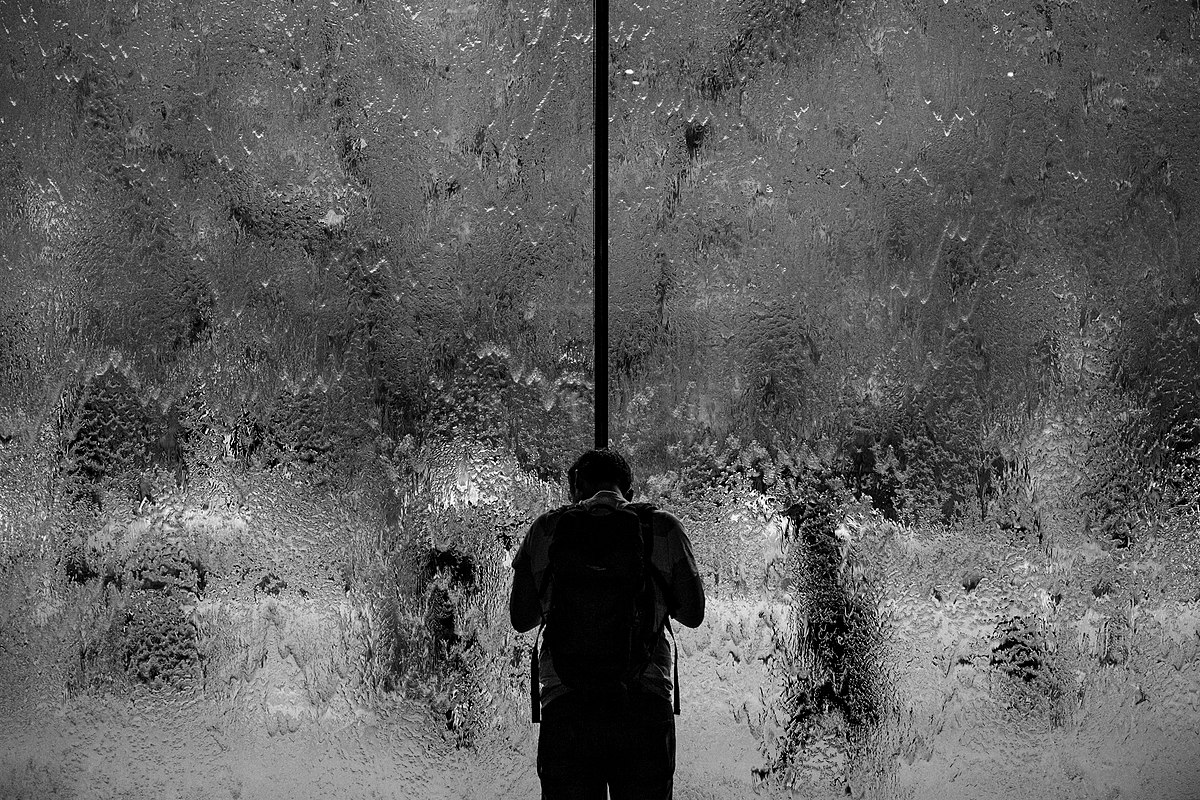
\includegraphics[width=.6\paperwidth]{window_water.jpg}
\end{center}

\begin{center}
\begin{minipage}[t]{0.7\paperwidth}\raggedright
\medskip
  
{\huge Dérive Comix}
\bigskip

\Large
\textbf{Context} you want to develop some future scenarios to explore with a group.\newline
\textbf{If} you have an group BUT everyone has their own experiences;\newline
\textbf{Then} Go for a walk or just look out the window wherever you, and document what you see. Follow up by preparing your materials to share in a succinct fashion, e.g., as photos, a screenshot, slides, sketches, a zine, a map, or some PostIt\textsuperscript{\textregistered} notes.\newline
% \textbf{Example} the Next Generation Services project (\url{http://nextgenpsf.co.uk}) used participatory scenario planning to imagine different plausible AI futures, which were then used in design sprints to expose professional services firms to potential AI challenges and opportunities.
\end{minipage}
\end{center}
\caption*{Image: Black and white shot of man from behind standing near of window covered in water, Melbourne.  Photograph by Sam Austin.  Public domain via Wikimedia commons.\newline 
\url{https://commons.wikimedia.org/wiki/File:Window_with_water_and_man_(Unsplash).jpg}}
\end{adjustbox}
\end{figure}

%%%

\begin{figure}[p]
\begin{adjustbox}{minipage=[c]{\textwidth-10mm},margin= 5mm 15mm 5mm 15mm, frame=1pt, bgcolor=almond,env=center}%
\begin{center}
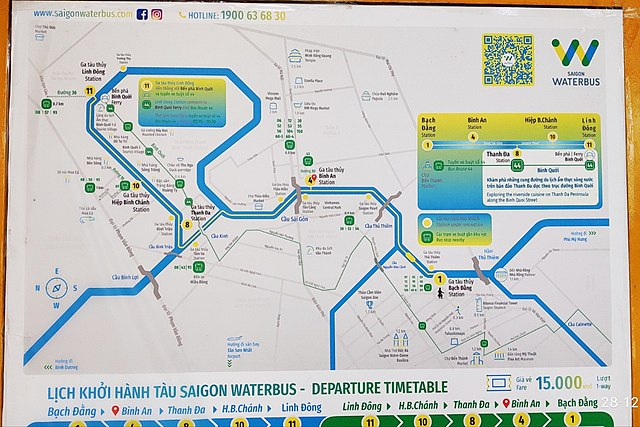
\includegraphics[trim=10mm 20mm 13mm 10mm, clip,width=.7\paperwidth]{Saigon.jpg}
\end{center}
\begin{center}
\begin{minipage}[t]{0.7\paperwidth}\raggedright
\medskip

{\huge Meaning Map}
\bigskip

\Large
\textbf{Context} We have collected images describing people’s worlds (see {\sc Dérive Comics}).\newline
\textbf{If} you want to distill shared meaning BUT everyone has their own experience;\newline
\textbf{Then} talk together about the problems and opportunities that everyone sees.  Maybe some of these will cluster together, or maybe everyone will have their own different perspective: that’s OK.  You can use these different viewpoints to get everyone on the same map.\newline\smallskip

%\textbf{Example} a bipartisan group of politicians, former civilian and military officials, and academics gathered to play a scenario planning game to anticipate the possible aftermath of a contested election: at the very least the scenarios they came up with managed to surprise them (Bidgood, 2020).

\end{minipage}
\end{center}
\caption*{Image: Sai Gon Water Bus - Line 1 map in the Binh An station.  Public domain
via Wikimedia Commons).\newline
\url{https://commons.wikimedia.org/wiki/File:Sai_Gon_Water_Bus_-_Line_1_map_in_the_Binh_An_station.jpg}}
\end{adjustbox}
\end{figure}

%%%

\begin{figure}[h]
\begin{adjustbox}{minipage=[c]{\textwidth-10mm},margin= 5mm 5mm 5mm 5mm, frame=1pt, bgcolor=almond,env=center}%
\begin{center}
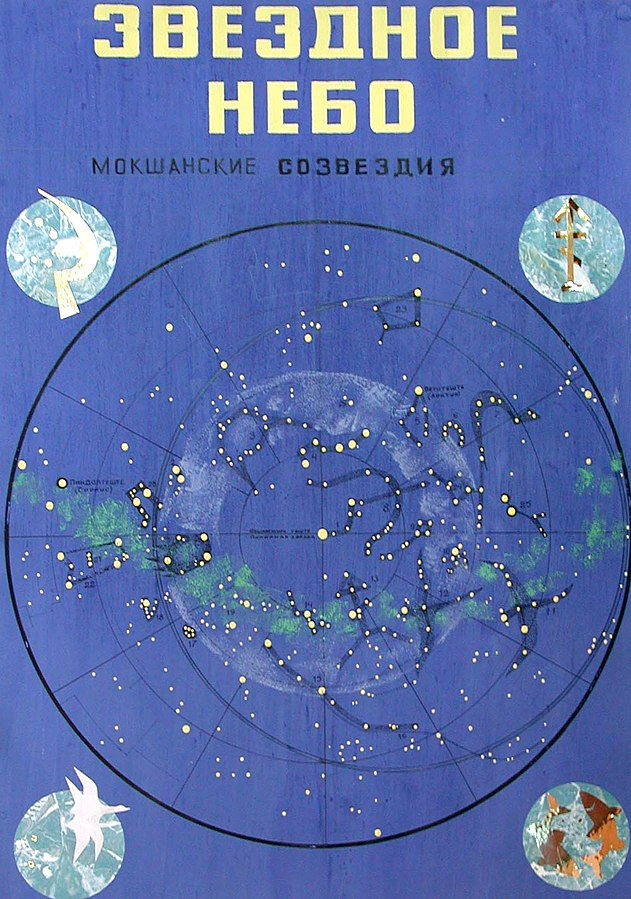
\includegraphics[trim=0mm 0mm 0mm 65mm, clip,  width=.78\columnwidth]{star_chart.jpg}
\end{center}
\begin{center}
\begin{minipage}[t]{0.97\columnwidth}\raggedright
\medskip
{\huge Reinfuse Expertise}
\bigskip

\Large
\textbf{Context} a group wants to build a {\sc Meaning Map}.\newline
\textbf{If} everyone has experience as a citizen BUT they also have expertise;\newline
\textbf{Then} begin by removing expertise to get everyone on the same page, and subsequently reinfuse expertise to enable richer and more complex thinking.\newline\smallskip
\bigskip

%\textbf{Example} Everyday roadmap languages include both iconic map and road sign symbols; when people are confused or lost they may ask for help or try to find their own way back to the road using other informal languages.
\end{minipage}
\end{center}

\caption*{Image: Old Moksha Star Map used by travellers and navigators in Middle ages.  Public domain via Wikimedia
Commons\newline
\url{https://commons.wikimedia.org/wiki/File:Medieval_Moksha_Star_Chart.jpg}}
\end{adjustbox}
\end{figure}

\end{document}